\chapter{Korišteni algoritmi i matematički aparat}

\section{Funkcije gubitka}

Gubitak je funkcija koja nam govori koliko nam je model dobar u predviđanju na skupu za učenje. Njega nastojimo minimizirati nekim od optimizacijskih postupaka. Postoje različite vrste gubitaka koje nam mogu dati različite rezultate za isti model. Neke od najpoznatijih funkcija gubitaka su: Unakrsna entropija (engl. Cross Entropy) i Negativna log izglednost (engl. Negative log likelihood). Minimizacija gubitka je iterativan postupak koji svakom iteracijom pomiče parametre modela u smjeru smanjenja gubitka.

\subsection{Negativna log-izglednost}
	Negativna log-izglednost je gubitak izražen formulom:
	\[
		L = -\sum_{i}log P(Y = y_i | \textbf{x}_i)
	\]
	$P(Y = y_i | \textbf{x}_i)$ je vjerojatnost da se podatak $\textbf{x}_i$ klasificira u razred $y_i$.
	Tu vjerojatnost računamo pomoću softmaxa. Softmax je funkcija koja "spljošćuje" ocjenu svakog podatka na interval [0,1].
	\[
	S : \mathbb{R} \mapsto [0,1]
	\]
	\[
	S(f_{y_i}) = \frac{e^{f_{y_i}}}{\sum_{j} e^{f_j}}
	\]
	Ovakva formulacija nam osigurava da će suma svih softmaksa primijenjenih na ocjene biti 1. Iz slike \ref{fig:NLL} vidimo kako negativna log-izglednost penalizira male vjerojatnosti, dok je za vjerojatnosti koje su blizu 1 gubitak približan nuli.
	\begin{figure}[H]
		\centering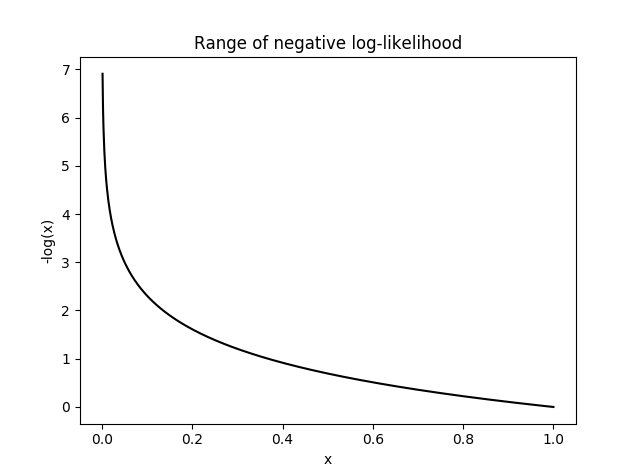
\includegraphics[scale=0.5]{slike/neg_log.png}
		\caption{NLL}
		\label{fig:NLL}
	\end{figure}

\subsection{Udaljenost od naučenih središta}
	Udaljenost od naučenih središta je gubitak izražen formulom:
	\[
		L_c = \frac{1}{2} (x_i-c_k)^2
	\]
	\[
		c_k = \frac{1}{N_k}\sum_{y_i=k}f_{y_i}^1(x_i)
	\]
	$c_k$ - središta klasa
	\newline
	$x_i$ - podatak
	\newline
	$f_{y_i}^1(x_i)$ - izlazi iz mreže
	\newline
	
Ovaj gubitak nastoji minimizirati udaljenosti izlaznih podataka od središta pripadnih razreda. Posljedica tog pristupa je bolje grupiranje podataka koji pripadaju istom razredu. Najčešće se koristi u kombinaciji s nekim drugim gubitkom npr. negativnom log-izglednosti, pri čemu se utjecaj ovog gubitka skalira nekim parametrom radi stabilnosti. Ovakav pristup smo odabrali u projektu te funkcija gubitka izgleda ovako.
\[
	L = L_n + \lambda L_c
\]
 Ovaj gubitak pokazuje najbolje rezultate u slučaju kad podatci za učenje sadrže mali broj slika po razredu, a veliki broj razreda.
	 


\section{Backpropagation}

backprop

\section{Momentum}

momentum

\section{Optimizatori}

\subsection{Stochastic gradient descent}

sgd

\subsection{Adam}

adam